\subsection{Time Domain Requirements}
The step response displays the time behaviour of the system when given an impulse. \autoref{fig:GIR} shows an example of a step response of a dynamic system.

\begin{figure}[H]
\centering
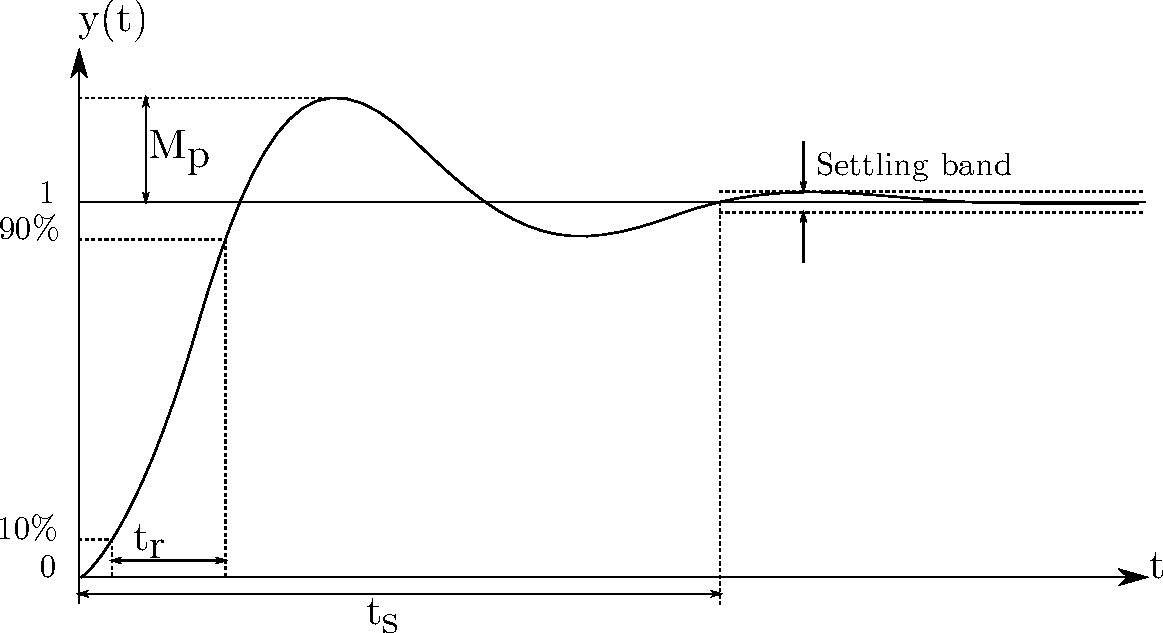
\includegraphics[width = 0.8\textwidth]{figures/steprequ.pdf}
\caption{General step response in time domain. } 
\label{fig:GIR}
\end{figure}
In \autoref{fig:GIR}, the variable $t_r$ is the rise time, defined as the time it takes for the step response to go from 10\% to 90\% of the step. The settling time, $t_s$, describes the time it takes for the system to settle within a certain margin of the final value, typically 1\%, 2\% or 5\%. The steady state error is the difference between the desired steady state value, and the actual steady state value. 
%The variable $t_p$, is the time it takes for the system to reach its maximum value, also called the peak time.
The ratio between the step response's ideal level and the maximum level which the system reaches is the overshoot, $M_p$.\\
To make sure the control system is stable, the system should not have any poles in the right-half-plane of the s-plane \citep[p. 146]{sou:Feedback}, or any poles outside the unit circle, if considering the z-plane \citep[p. 619]{sou:Feedback}.
\\\\
It is desirable not to have a steady-state error, as the balancing of the segway shall be as accurate as possible, to ensure that the angle the segway is to maintain is also met, as an steady-state error in the inverted pendulum angle will cause the segway to move forward or backwards.
It is likewise desirable to have a fast rise time, as it would decrease the risk of the segway of falling over if the controller regulates the segway to an upright balanced position quickly. However, this will result in an overshoot, as the system's quick response to the impulse, for example a push, will make the system overcompensate to minimize the error quickly. This will increase the risk of the segway of falling over, if the overshoot is so high that the segway falls to the other side. The overshoot can also cause oscillations, if the controller constantly tries to obtain the desired angle, but has an overshoot so high, that the overshoot angle also has to be corrected by the controller. Disturbances to the controller making the system unstable, such as the gravity, can affect the way the segway moves forward at a steady velocity. It is important to reduce both disturbances and noise affecting the sensor values, to obtain a control system with high precision.\\
The segway's balance controller shall thus, as with any control system, be a compromise of an agile behaviour, where the settling time is not too long and where overshoot is limited.

The step response is a useful means of evaluating the dynamics of a system, i.e. the rise and settling time, the overshoot and the steady state error. The step is applied to the closed loop, as the step response then includes the effect of the feedback.

The general transfer function for the basic closed loop feedback system is shown in \autoref{eq:GCL} and the corresponding block diagram is shown in \autoref{fig:GCL}. 

\begin{equation}
T(s) = \frac{Y(s)}{R(s)} = \frac{\text{Direct term}}{1 + \text{Open loop}}
\label{eq:GCL}
\end{equation}
%\begin{where}
%\punkt{$T(s)$}{function for closed loop magnitude in s domain}{dB}
%\punkt{$Y(s)$}{function for output signal}{dB}
%\punkt{$R(s)$}{function for input signal}{dB}
%\punkt{$D(s)$}{function for controller}{dB}
%\punkt{$G(s)$}{function for plant}{dB}
%\punkt{$H(s)$}{function for sensor}{dB}
%\end{where}

\begin{figure}[H]
\centering
\input{figures/GeneralClosedLoop.ralf}
\caption{Block diagram of a general closed loop feedback system.}
\label{fig:GCL}
\end{figure}

It is assumed that the system that is to be controlled is a second order stable closed loop system, on the form as listed in \autoref{TFgeneral}.
\begin{equation}
T(s)=\frac{A}{s^2 + 2\zeta\omega_n s + \omega_n^2}
\label{TFgeneral}
\end{equation}
\begin{where}
\va{$A$}{is the DC gain}{1}
\va{$\zeta$}{is the damping factor}{1}
\va{$\omega_n$}{is the natural frequency}{rad/s}
\end{where}

Due to this, the relationship between the different quantities can be expressed from the following rules of thumb \citep[p. 152]{sou:Feedback}:
\begin{align}
M_p &= \exp{\frac{-\pi \zeta}{\sqrt{1-\zeta^2}}} \label{overshoot}\\
t_r &\approx \frac{1.8}{\omega_n}\label{risetime}\\
t_s &= \frac{-\text{ln}(x)}{\zeta\omega_n}, x = \text{settling band, e.g. 0.01 for 1\%} \label{settlingtime}\\
\zeta &\approx \frac{PM}{100}\label{zeta}
\end{align}

Assuming that the system is 2nd order, it is thus possible to set up realistic requirements for the system based on these equations. First of, it is decided that no steady-state error is acceptable, as it will cause the pendulum to move forward at a steady velocity at all times, which is not desired.

It is chosen that the overshoot should be no more than 10\%, i.e. $M_p \leq 0.10$. Using \autoref{overshoot}, $\zeta$ is found to be equal to $\zeta = 0.8$. By deciding that the settling time $t_s$ should be less than 3 seconds for a 1 \% settling band, it is found that $\omega_n = 1.92$ using \autoref{settlingtime} and the found value for $\zeta$.
This can be inserted in \autoref{risetime}, giving a rise time of $t_r = 0.94 \, s$. This is considered acceptable, but to give some margin, the requirement is increased to 1 s. Thus, the requirements for the step response of the system has been determined. The requirements are summed up below.

Steady state error: 0 \%\\
Rise time: < 1 s\\
Settling time: < 3 s\\
Overshoot: $\leq$ 10 \% 

%The exact proportions can not be found from theory or rule of thumb, but instead determined from simulations and tests on a model of the system. The compromise of the three values, namely rise time, settling time and overshoot, will therefore not be determined at this point. There can be set some guidelines, to limit the simulations and tests. These guidelines is build upon rules of thumb and are evaluated and chosen by the projectgroup. \todo[inline]{not finnished, look besides it!}




%If the rise time is very large, the segway will not be able to stabilise itself before hitting the ground. The rise time is not the only variable in this matter. 
%The force applied by the push can be too large for the mini segway to arise from. The rise time neither be too short, as this would increase overshoot. By having a too large overshoot, the mini segway is more likely to fall if first pushed in one direction, then, as the mini segway enters overshoot, starts driving in the same direction.
%Thus the rise time should be determined as compromise between these two reasons.
%The overshoot should be as small as possible, since overshoot increases the risk of the mini segway to fall, when the mini segway is driving at changing speeds.
%The shorter the settling time and steady state error, the faster the segway stabilises itself at its upright position. Thus these variables should be as short as possible.

With requirements set up for the time domain response of the signal, it is now desired to set up requirements for the frequency domain. This is done by means of requirements to the phase and gain margin. 

%From the step response, the transfer function of the system can be found. The transfer function gives the phase and gain margin if plotted in a bodeplot. 